\documentclass[usepdftitle=false]{beamer}

\usepackage[french]{babel}
\usepackage[T1]{fontenc}
\usepackage[utf8]{inputenc}
\usepackage[labelformat=empty]{caption}

\usetheme{Warsaw}

\title{Data Defense}
\author[Serious Game]{Schmitt Clément \\ Brasseur Julien \\ Vinard Florian \\ Mathieu Alexandre}
\institute{Université Montpellier II}
\date{15 janvier 2014}

\addtobeamertemplate{navigation symbols}{}{%
    \usebeamerfont{footline}%
    \usebeamercolor[fg]{footline}%
    \hspace{1em}%
    \insertframenumber/\inserttotalframenumber
}

\begin{document}

	\begin{frame}
		\titlepage
	\end{frame}
	
	\begin{frame}
		\tableofcontents[hideallsubsections]
	\end{frame}
	
	\section{Introduction}
	\subsection{Quel type de jeu ?}
	\begin{frame}
		\begin{itemize}
			\item Gameplay : Tower Defense
			\item Thème : Vol de données sensibles dans le domaine de l'informatique
		\end{itemize}
	\end{frame}
	
	\subsection{Étude de l'existant}
	\begin{frame}		
		\begin{columns}[T]
			\begin{column}{5cm}
				\begin{figure}
    					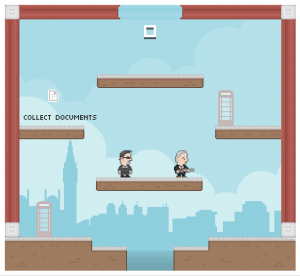
\includegraphics[scale=0.3]{wikigame.png}
    					\caption{{\tiny The Wikileaks Game, 2010}}
				\end{figure}
			\end{column}

			\begin{column}{5cm}
				\begin{figure}
    					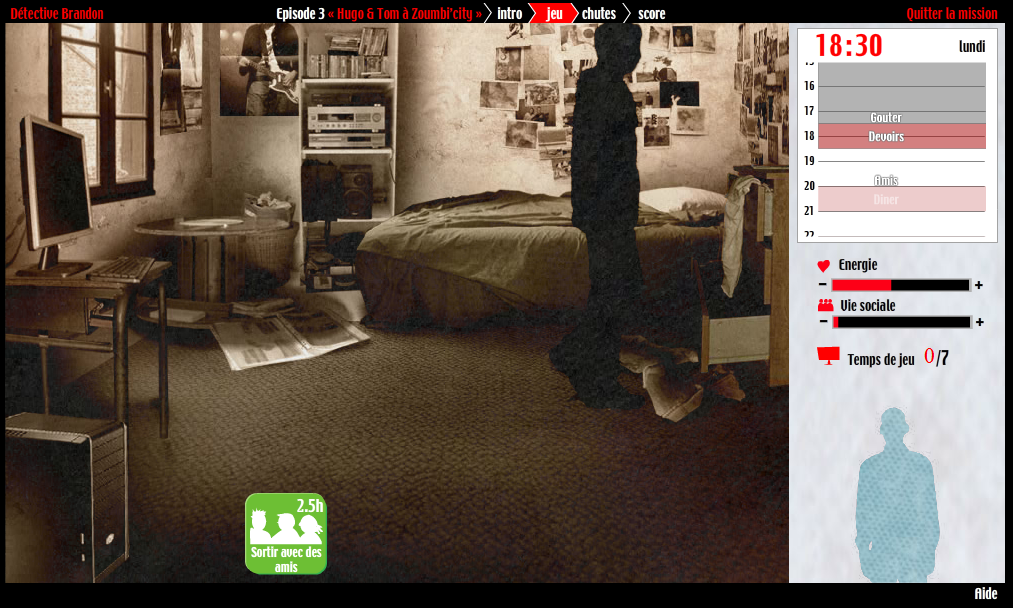
\includegraphics[scale=0.15]{exm.png}
    					\caption{{\tiny 2025 exmachina, 2010}}
				\end{figure}
			\end{column}
		\end{columns}
		
		\begin{columns}[T]
			\begin{column}{5cm}
				\begin{figure}
    					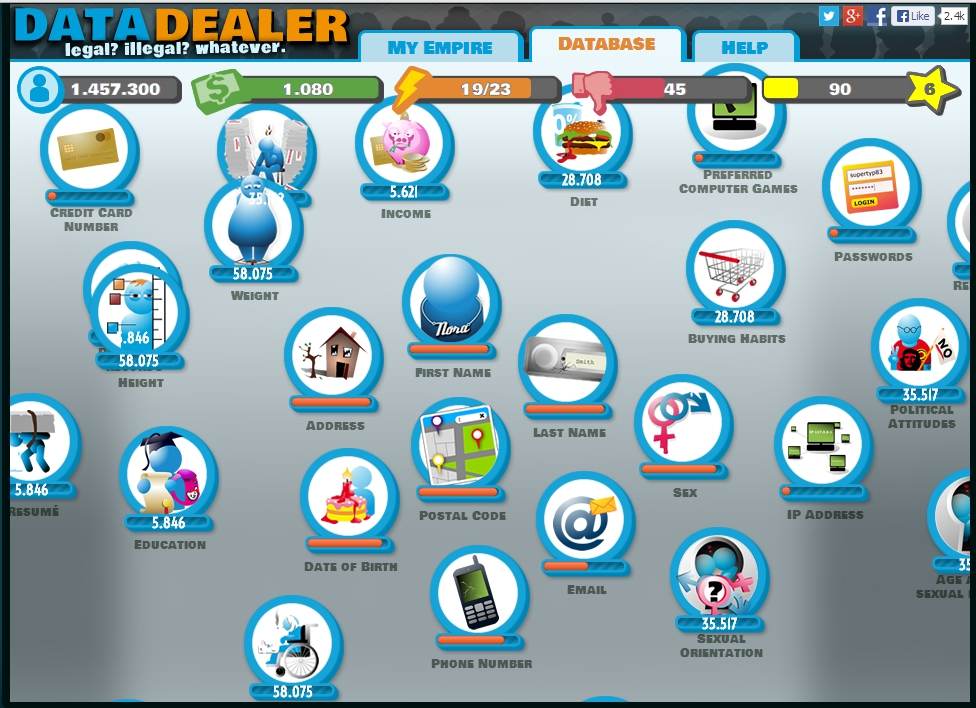
\includegraphics[scale=0.1]{datad.jpg}
    					\caption{{\tiny Data Dealer, 2013}}
				\end{figure}
			\end{column}

			\begin{column}{5cm}
				\begin{figure}
    					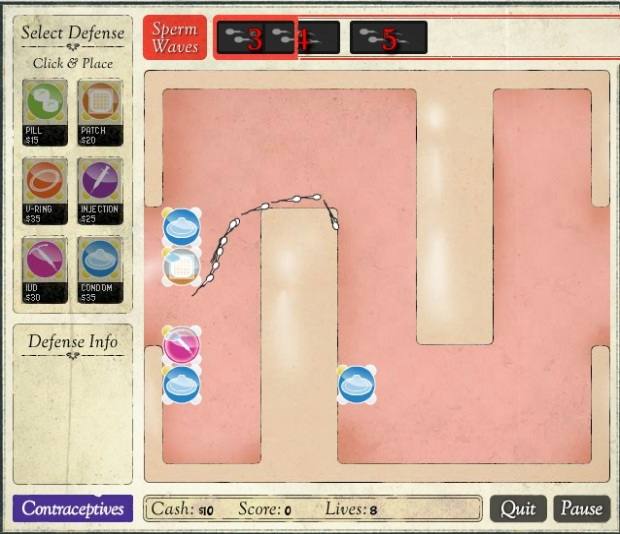
\includegraphics[scale=0.17]{sq.jpg}
    					\caption{{\tiny Sex Quest, 2012}}
				\end{figure}
			\end{column}
		\end{columns}
	\end{frame}
	
	\section{Gameplay}
		\begin{frame}
			\center
			\begin{itemize}
				\item \textbf{Objectif} : Protéger l'ensemble de ses données
				\item \textbf{Challenge} : Les ennemis volent les données
				\item \textbf{Récompense} : Abattre les ennemis procure de l'argent
				\item \textbf{Moyen} : L'argent permet de construire des tours et de les améliorer
			\end{itemize}
		\end{frame}
		
		\begin{frame}
			Victoire
			\begin{itemize}
				\item Le joueur survie a toutes les vagues d'ennemis
			\end{itemize}
			Défaite
			\begin{itemize}
				\item Le joueur ne possède plus aucunes données
			\end{itemize}
		\end{frame}
	
	\section{Le contenu sérieux}
	\subsection{Généralités}
	\begin{frame}
		\begin{itemize}
			\item Public
			\item Objectifs
			\item Activités
		\end{itemize}
	\end{frame}
	
	\begin{frame}
		Mise en place du thème
		\begin{figure}
			\center
    			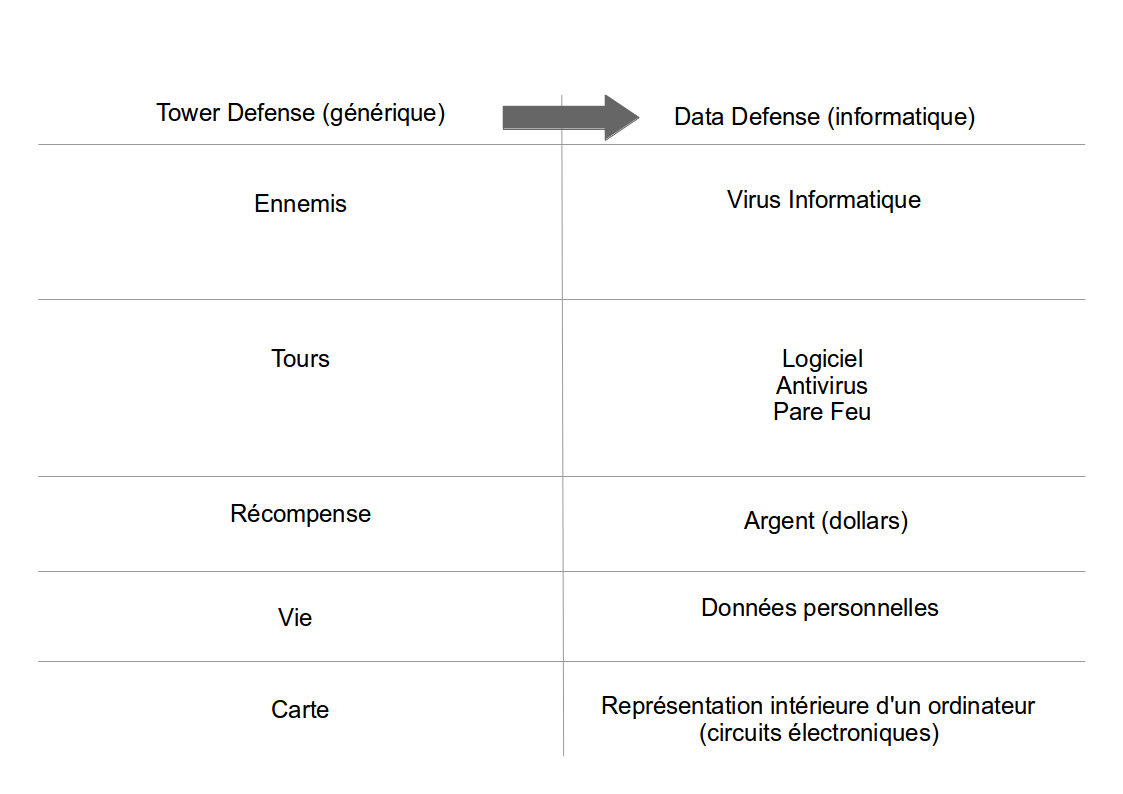
\includegraphics[scale=0.3]{adapt.png}
		\end{figure}
	\end{frame}
	
	\subsection{Sensibiliser le joueur}
	\begin{frame}
		\begin{itemize}
			\item Approche intrinsèque
			\item Accompagnement progressif
			\item Déclencher des mécanismes logique
			\item Sans comprendre les différents éléments du jeu, la victoire est difficilement accessible
			\item Reproduire des événements réels de façon ludique
		\end{itemize}
	\end{frame}
	
	\subsection{Les acteurs}
	\begin{frame}
	\begin{block}{Les ennemis}
  			Les virus volent ou corrompent les données personnelles du joueur.
 		\end{block}
 		\begin{block}{Les tours}
  			Les logiciels doivent empêcher les virus de voler ou corrompre les données.
 		\end{block}
 		Concernant les données
 		\begin{itemize}
			\item Si toutes les données du joueur ont été volées ou corrompues, le joueur a perdu
			\item Les données corrompues peuvent être récupérées en faisant un scan du système
		\end{itemize}
	\end{frame}
	
	\section{Réalisation}
	\begin{frame}
		\begin{itemize}
			\item Outils
		\end{itemize}
	\end{frame}
	
	\section{Conclusion}
	\begin{frame}
		\begin{itemize}
			\item Améliorations
			\item Diversification
		\end{itemize}
	\end{frame}

\end{document}